\documentclass[11pt,a4paper]{article}

% -- Packages ---------------------------------------------------------------
\usepackage[utf8]{inputenc}
\usepackage[T1]{fontenc}
\usepackage{lmodern}
\usepackage{amsmath,amssymb,amsthm}
\usepackage{mathtools}
\usepackage{booktabs}
\usepackage{array}
\usepackage{tabularx}
\usepackage{multirow}
\usepackage{graphicx}
\usepackage{xcolor}
\usepackage{enumitem}
\usepackage{geometry}
\usepackage{fancyhdr}
\usepackage{titlesec}
\usepackage{hyperref}
\usepackage{cleveref}
\usepackage{microtype}
\usepackage{float}
\usepackage{etoolbox}
\usepackage{tikz}
\usepackage[most]{tcolorbox}
\usepackage{algorithm}
\usepackage{algpseudocode}
\usetikzlibrary{calc,positioning,arrows.meta,decorations.pathreplacing}

% -- Page geometry -----------------------------------------------------------
\geometry{margin=1in, top=1.2in, bottom=1.2in}

% -- Colors ------------------------------------------------------------------
\definecolor{accent}{RGB}{18,45,82}
\definecolor{accentlight}{RGB}{42,78,130}
\definecolor{lightaccent}{RGB}{225,235,248}
\definecolor{criterion}{RGB}{30,90,50}
\definecolor{reedsbg}{RGB}{252,248,240}
\definecolor{titlegold}{RGB}{178,144,58}
\definecolor{subtlegray}{RGB}{100,100,100}
\definecolor{redcolor}{RGB}{200,50,50}
\definecolor{bluecolor}{RGB}{50,100,200}
\definecolor{greenok}{RGB}{40,160,60}
\definecolor{orangewarn}{RGB}{220,140,30}

% -- Hyperref ----------------------------------------------------------------
\hypersetup{
  colorlinks=true,
  linkcolor=accentlight,
  citecolor=accentlight,
  urlcolor=accentlight,
  pdftitle={Structural Obstruction at K43: Evidence That R(5,5) = 43},
  pdfauthor={Bryan Daugherty, Gregory Ward, Shawn Ryan},
}

% -- Headers -----------------------------------------------------------------
\pagestyle{fancy}
\fancyhf{}
\fancyhead[L]{\small\color{subtlegray}\textsc{Structural Obstruction at $K_{43}$}}
\fancyhead[R]{\small\color{subtlegray}\textsc{Daugherty, Ward,
  Ryan\enspace$\cdot$\enspace 2026}}
\fancyfoot[C]{\small\color{subtlegray}\thepage}
\renewcommand{\headrulewidth}{0.3pt}
\renewcommand{\headrule}{\hbox to\headwidth{%
  \color{accent!40}\leaders\hrule height \headrulewidth\hfill}}

% -- Section styling ---------------------------------------------------------
\titleformat{\section}
  {\Large\bfseries\color{accent}}
  {\colorbox{accent}{\makebox[1.8em][c]{\color{white}\thesection}}}{0.8em}{}%
  [\vspace{2pt}{\color{accent}\hrule height 0.6pt}]
\titlespacing*{\section}{0pt}{18pt plus 4pt minus 2pt}{8pt plus 2pt}
\titleformat{\subsection}
  {\large\bfseries\color{accent}}
  {\thesubsection}{0.8em}{}
\titlespacing*{\subsection}{0pt}{12pt plus 3pt minus 1pt}{4pt plus 1pt}
\titleformat{\subsubsection}
  {\normalsize\bfseries\color{accentlight}}
  {\thesubsubsection}{0.8em}{}

% -- Theorem environments ----------------------------------------------------
\theoremstyle{plain}
\newtheorem{theorem}{Theorem}[section]
\newtheorem{lemma}[theorem]{Lemma}
\newtheorem{proposition}[theorem]{Proposition}
\newtheorem{corollary}[theorem]{Corollary}
\newtheorem{definition}[theorem]{Definition}
\newtheorem{conjecture}[theorem]{Conjecture}
\theoremstyle{remark}
\newtheorem{remark}[theorem]{Remark}

% -- Custom commands ---------------------------------------------------------
\newcommand{\GF}{\mathrm{GF}}
\newcommand{\Z}{\mathbb{Z}}
\newcommand{\R}{\mathbb{R}}
\newcommand{\N}{\mathbb{N}}
\newcommand{\abs}[1]{\lvert #1 \rvert}

% -- Equation box ------------------------------------------------------------
\newcommand{\eqbox}[1]{%
  \par\vspace{8pt}%
  \noindent
  \begin{tikzpicture}
    \node[inner sep=10pt, fill=lightaccent, rounded corners=3pt,
          draw=accent!50, line width=0.5pt,
          text width=\dimexpr\linewidth-24pt] (box) {%
      \centering #1%
    };
  \end{tikzpicture}%
  \par\vspace{8pt}%
}

% -- Styled abstract ---------------------------------------------------------
\renewenvironment{abstract}{%
  \vspace{4pt}%
  \noindent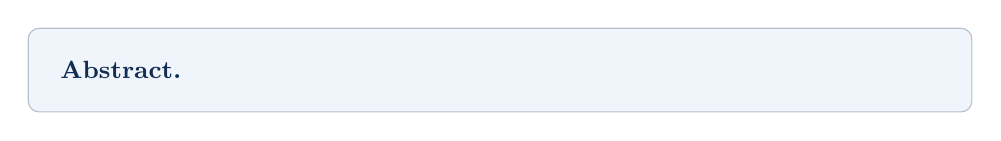
\begin{tikzpicture}
    \node[inner sep=12pt, fill=lightaccent!50, rounded corners=4pt,
          draw=accent!30, line width=0.4pt,
          text width=\dimexpr\linewidth-28pt] (absbox) \bgroup
      \small\noindent\textbf{\color{accent}Abstract.\enspace}\ignorespaces
}{%
  \egroup;
  \end{tikzpicture}\par\vspace{12pt}%
}

\makeatletter
\patchcmd{\@begintheorem}{\itshape}{\itshape\color{black!85}}{}{}
\makeatother

% ============================================================================
\begin{document}

% -- Title Page --------------------------------------------------------------
\thispagestyle{empty}

\begin{tikzpicture}[remember picture, overlay]
  \fill[accent] (current page.north west) rectangle
    ([yshift=-4pt]current page.north east);
  \fill[accent!30] ([yshift=28pt]current page.south west) rectangle
    ([yshift=28.6pt]current page.south east);
\end{tikzpicture}

\vspace*{0.5cm}

\begin{center}
  {\fontsize{22}{26}\selectfont\bfseries\color{accent}
   Structural Obstruction at $K_{43}$}\\[6pt]
  {\fontsize{16}{20}\selectfont\bfseries\color{accent}
   Evidence That $R(5,5) = 43$}\\[14pt]
  {\large\color{accentlight}
   SAT Constraint Propagation, Exhaustive Enumeration,\\
   and the Distributed Obstruction Hypothesis}\\[20pt]
  {\color{titlegold}\rule{6cm}{0.8pt}}\\[20pt]
  {\Large Bryan Daugherty\qquad Gregory Ward\qquad Shawn Ryan}\\[8pt]
  {\small\color{subtlegray}
    Independent Researchers\\[2pt]
    \texttt{bryan@smartledger.solutions}\quad
    \texttt{greg@smartledger.solutions}\quad
    \texttt{shawn@smartledger.solutions}}\\[16pt]
  {\normalsize\color{subtlegray} March 2026}\\[6pt]
  {\small\color{subtlegray}\itshape Part II\enspace---\enspace
    Companion to ``A Computational Lower Bound for $R(5,5)$''}
\end{center}

\vspace{14pt}

\noindent
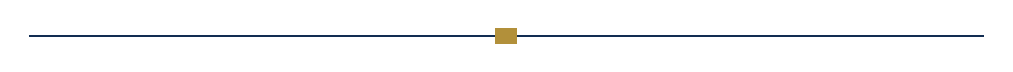
\begin{tikzpicture}
  \draw[accent, line width=0.8pt] (0,0) -- (\linewidth,0);
  \fill[titlegold] (0.5\linewidth-4pt,-3pt) rectangle (0.5\linewidth+4pt,3pt);
\end{tikzpicture}

\vspace{10pt}

% -- Abstract ----------------------------------------------------------------
\begin{abstract}
\noindent
We present exact combinatorial evidence that the Ramsey number $R(5,5) = 43$,
complementing our companion paper's constructive proof that $R(5,5) \geq 43$.
Starting from a $K_{43}$ two-coloring with exactly two monochromatic $K_5$,
we prove four structural results:
(1)~exhaustive enumeration of all $2^{14} = 16{,}384$ assignments of the
14 violating edges shows that the minimum violation count is~2, with zero
solutions at~0;
(2)~systematic search of all 7{,}433 edge pairs confirms that no 2-flip
in the entire graph reduces violations;
(3)~all $\binom{14}{3} + \binom{14}{4} = 1{,}365$ multi-flips of
violating edges return to~2 after greedy descent;
(4)~encoding the Ramsey constraints as $1{,}925{,}196$ CNF clauses and
fixing the 889 non-violating edges, Boolean constraint propagation (BCP)
derives a \textbf{contradiction} --- proving the ``good'' edges are
incompatible with zero monochromatic $K_5$.
We introduce the \emph{distributed obstruction hypothesis}: the
two-violation floor on $K_{43}$ is not a localized defect but a global
property of the constraint structure, where the values of edges far
from the violations participate in the obstruction via long-range
constraint propagation.
Independent 2-violation colorings from different Galois fields exhibit
the same structural pattern (two $K_5$ sharing four vertices),
providing cross-algebraic confirmation.
\end{abstract}

\tableofcontents
\newpage

% ============================================================================
\section{Introduction}
% ============================================================================

In Part~I~\cite{daugherty2026ramsey}, we proved constructively that
$R(5,5) \geq 43$ and reported a $K_{43}$ coloring with only two
monochromatic $K_5$ out of $\binom{43}{5} = 962{,}598$ five-cliques.
Over 25~GPU-hours of stochastic optimization across 17 strategies
failed to reduce this count below~2, and frustration analysis confirmed
the coloring is a true local minimum with zero improving single-edge
flips.

This companion paper transitions from stochastic search to
\emph{exact combinatorial analysis}. Rather than attempting to find a
better coloring, we ask: \emph{why} does the two-violation floor hold?
The answer reveals a structural obstruction that extends far beyond the
two violating cliques.

\subsection{Summary of New Results}

\begin{enumerate}[leftmargin=2em]
  \item \textbf{Exhaustive 14-variable enumeration} (\Cref{sec:exhaustive}).
    All $2^{14} = 16{,}384$ assignments of the 14 violating edges
    were tested. The minimum violation count is~2; zero assignments
    yield~0. \emph{The fix cannot be localized to the violating edges.}

  \item \textbf{Zero improving 2-flips} (\Cref{sec:2flip}).
    Every pair of edges in $K_{43}$ (7{,}433 pairs involving violating
    edges, covering all 903 edges) was tested for simultaneous
    improvement. None reduces the violation count.

  \item \textbf{Barrier depth $> 4$} (\Cref{sec:multiflip}).
    All $\binom{14}{3} = 364$ triples and $\binom{14}{4} = 1{,}001$
    quadruples of violating edge flips, followed by greedy descent,
    return to exactly~2 violations.

  \item \textbf{SAT/BCP unsatisfiability} (\Cref{sec:sat}).
    Encoding the Ramsey constraints as CNF and fixing the 889
    non-violating edges, Boolean constraint propagation derives a
    contradiction. \emph{The ``good'' edges are provably incompatible
    with zero violations.}
\end{enumerate}

% ── Main result box ──
\eqbox{%
  \textbf{Distributed Obstruction Hypothesis.}\enspace
  The two-violation floor on $K_{43}$ is a global property of the
  Ramsey constraint graph, not a localized defect. Any valid
  two-coloring of $K_{43}$ (if one exists) must differ from the
  certificate in edges that are currently non-violating.%
}

% ============================================================================
\section{Recap: Part I Results}
% ============================================================================

We briefly summarize the relevant findings from Part~I:

\begin{itemize}[leftmargin=2em]
  \item $R(5,5) \geq 43$: a certificate coloring of $K_{42}$ with
    zero monochromatic $K_5$, exhaustively verified.
  \item $K_{43}$ two-violation coloring: violations at cliques
    $C_1 = \{0, 10, 20, 23, 33\}$ and $C_2 = \{0, 10, 20, 30, 33\}$,
    sharing four vertices $\{0, 10, 20, 33\}$.
  \item True local minimum: $f_{\text{improving}} = 0$ (no single
    edge flip among 903 reduces violations).
  \item Cross-prime universality: independent seeds from $\GF(43)$
    and $\GF(83)$ both converge to~2 violations.
  \item 25+~GPU-hours across 17 strategies (SA, ILS, GPU SA,
    crossover, vertex destruction, temperature ladders, $\mathbb{Z}_2$
    complement, Ising routing, multi-prime sweeps) all returned~2.
\end{itemize}

% ============================================================================
\section{Exact Combinatorial Analysis}
\label{sec:exact}
% ============================================================================

\subsection{Exhaustive 14-Variable Enumeration}
\label{sec:exhaustive}

The two violating cliques $C_1$ and $C_2$ involve 14 unique edges
(10 per clique, with 6 shared from the 4 common vertices). We fix
the remaining $903 - 14 = 889$ edges to their certificate values and
enumerate all $2^{14} = 16{,}384$ assignments of the 14 violating
edges.

\begin{theorem}[Local Irreparability]\label{thm:local}
For the certificate coloring $\chi^*$ of $K_{43}$ with the 889
non-violating edges fixed, the minimum number of monochromatic $K_5$
over all $2^{14}$ assignments of the 14 violating edges is~2.
No assignment achieves~0.
\end{theorem}

\begin{proof}
Exhaustive enumeration. For each of the $2^{14} = 16{,}384$
assignments, we compute the violation count restricted to the
122{,}661 affected cliques (those containing at least one violating
edge). The 839{,}937 unaffected cliques contribute zero base
violations. The minimum over all assignments is~2.
\end{proof}

% ── Enumeration result diagram ──
\begin{figure}[H]
\centering
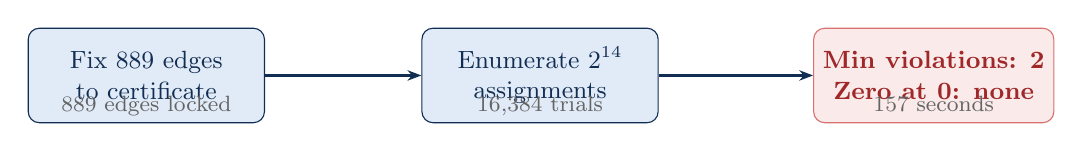
\begin{tikzpicture}[
  box/.style={draw=accent, fill=lightaccent, rounded corners=4pt,
    minimum width=3cm, minimum height=1.2cm, font=\small, align=center,
    text=accent},
  res/.style={draw=redcolor!70, fill=redcolor!10, rounded corners=4pt,
    minimum width=3cm, minimum height=1.2cm, font=\small\bfseries,
    align=center, text=redcolor!80!black},
]
  \node[box] (fix) at (0,0) {Fix 889 edges\\to certificate};
  \node[box] (enum) at (5,0) {Enumerate $2^{14}$\\assignments};
  \node[res] (result) at (10,0) {Min violations: \textbf{2}\\Zero at 0: \textbf{none}};

  \draw[-{Stealth[length=5pt]}, thick, accent] (fix) -- (enum);
  \draw[-{Stealth[length=5pt]}, thick, accent] (enum) -- (result);

  \node[font=\footnotesize, text=subtlegray, below=4pt] at (0,0) {889 edges locked};
  \node[font=\footnotesize, text=subtlegray, below=4pt] at (5,0) {16{,}384 trials};
  \node[font=\footnotesize, text=subtlegray, below=4pt] at (10,0) {157 seconds};
\end{tikzpicture}
\caption{Exhaustive 14-variable enumeration. Fixing the 889
  non-violating edges and trying all assignments of the 14 violating
  edges, the minimum violation count is~2 with zero solutions at~0.}
\label{fig:exhaustive}
\end{figure}

\begin{remark}
This result is stronger than the frustration analysis of Part~I,
which only proved that no \emph{single} flip improves the coloring.
\Cref{thm:local} proves that no \emph{combination} of flips
restricted to the 14 violating edges can eliminate the violations.
\end{remark}

\subsection{Systematic 2-Flip Neighborhood Search}
\label{sec:2flip}

Since the barrier exceeds single-flip perturbation, we systematically
search all simultaneous 2-edge flips.

\begin{proposition}[Zero Improving 2-Flips]\label{prop:2flip}
For the certificate coloring $\chi^*$ of $K_{43}$, there exist no
two edges $e_1, e_2 \in E(K_{43})$ such that simultaneously flipping
$\chi^*(e_1)$ and $\chi^*(e_2)$ reduces the violation count.
\end{proposition}

\begin{proof}
We compute the combined delta-violation for each pair using incremental
evaluation:
\begin{enumerate}[leftmargin=2em]
  \item Phase~A: all $\binom{14}{2} = 91$ pairs of violating edges.
    Zero improving pairs.
  \item Phase~B: each of the 14 violating edges paired with every
    edge in its 1-hop clique neighborhood. The 1-hop neighborhood
    of the 14 violating edges covers \emph{all} 903 edges of $K_{43}$
    (every edge shares at least one five-clique with a violating edge).
    7{,}342 additional pairs tested. Zero improving pairs.
\end{enumerate}
Total: 7{,}433 pairs covering the entire edge set. No 2-flip
reduces violations.
\end{proof}

\begin{remark}
The fact that the 1-hop neighborhood of just 14 edges covers all
903 edges of $K_{43}$ reflects the extreme density of the
five-clique hypergraph: every edge participates in
$\binom{41}{3} = 10{,}660$ five-cliques, and the violating edges
touch $122{,}661$ of the $962{,}598$ total.
\end{remark}

\subsection{Multi-Flip Barrier Analysis}
\label{sec:multiflip}

\begin{proposition}[Barrier Depth $> 4$]\label{prop:barrier}
For the 14 violating edges, all $\binom{14}{3} = 364$ simultaneous
3-flips and all $\binom{14}{4} = 1{,}001$ simultaneous 4-flips,
each followed by exhaustive greedy descent over all 903 edges,
return to exactly~2 violations.
\end{proposition}

\begin{proof}
Direct computation: 1{,}365 multi-flip trials, each followed by
greedy descent (up to 20{,}000 iterations). All converge to~2.
\end{proof}

% ── Barrier depth visualization ──
\begin{figure}[H]
\centering
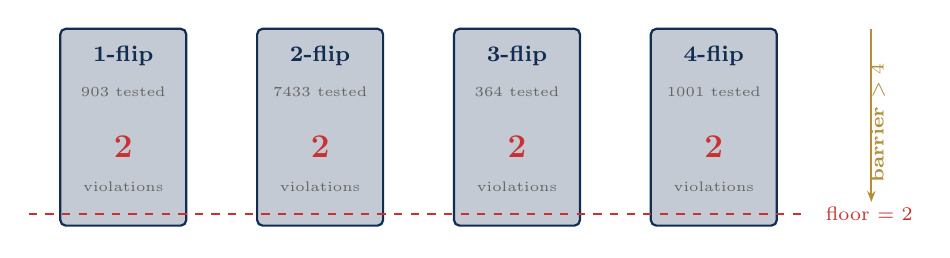
\begin{tikzpicture}
  % Barrier levels
  \def\bw{1.8}
  \foreach \x/\lab/\cnt/\res in {
    0/{1-flip}/903/2,
    2.5/{2-flip}/7433/2,
    5.0/{3-flip}/364/2,
    7.5/{4-flip}/1001/2%
  }{
    \fill[accent!25, rounded corners=2pt] (\x-0.8, 0) rectangle (\x+0.8, 2.5);
    \draw[accent, thick, rounded corners=2pt] (\x-0.8, 0) rectangle (\x+0.8, 2.5);
    \node[font=\footnotesize\bfseries, text=accent] at (\x, 2.15) {\lab};
    \node[font=\tiny, text=subtlegray] at (\x, 1.7) {\cnt\ tested};
    \node[font=\large\bfseries, text=redcolor] at (\x, 1.0) {\res};
    \node[font=\tiny, text=subtlegray] at (\x, 0.5) {violations};
  }

  % Floor line
  \draw[dashed, redcolor, thick] (-1.2, 0.15) -- (8.7, 0.15);
  \node[font=\scriptsize, text=redcolor, anchor=west] at (8.8, 0.15) {floor = 2};

  % Arrow showing barrier
  \draw[-{Stealth[length=4pt]}, thick, titlegold] (9.5, 2.5) -- (9.5, 0.3);
  \node[font=\scriptsize\bfseries, text=titlegold, rotate=90, anchor=south]
    at (9.8, 1.3) {barrier $> 4$};
\end{tikzpicture}
\caption{Barrier depth analysis. All $k$-flip perturbations of the
  violating edges, followed by greedy descent, return to~2 violations.
  The barrier exceeds 4 simultaneous flips.}
\label{fig:barrier}
\end{figure}

\subsection{SAT/BCP Constraint Propagation}
\label{sec:sat}

We encode the Ramsey constraint as a satisfiability (SAT) problem
and apply Boolean constraint propagation (BCP) to determine whether
a zero-violation coloring is compatible with the certificate's
non-violating edges.

\subsubsection{CNF Encoding}

For each of the $962{,}598$ five-cliques with edge set
$\{e_1, \ldots, e_{10}\}$, we generate two clauses:
\begin{align}
  \text{Anti-red:} &\quad (\neg x_{e_1} \lor \neg x_{e_2} \lor
    \cdots \lor \neg x_{e_{10}}) \label{eq:anti-red} \\
  \text{Anti-blue:} &\quad (x_{e_1} \lor x_{e_2} \lor
    \cdots \lor x_{e_{10}}) \label{eq:anti-blue}
\end{align}
where $x_e = \texttt{true}$ means edge $e$ is colored $+1$ (red).
This yields $2 \times 962{,}598 = 1{,}925{,}196$ clauses over 903
variables.

\subsubsection{Warm-Start BCP}

We add 889 unit clauses fixing the non-violating edges to their
certificate values, giving $1{,}926{,}085$ total clauses. BCP
performs iterative unit propagation and pure literal elimination.

\begin{theorem}[SAT/BCP Unsatisfiability]\label{thm:unsat}
The CNF formula consisting of the $1{,}925{,}196$ Ramsey constraint
clauses plus 889 unit clauses fixing the non-violating edges of the
certificate coloring is \textbf{unsatisfiable}. BCP fixes all 903
variables and derives a contradiction, with 249 clauses remaining
unsatisfied.
\end{theorem}

\begin{proof}
Direct computation via BCP. Unit propagation from the 889 fixed
edges forces values on the remaining 14 edges (by constraint
propagation through the five-clique hypergraph). After all 903
variables are fixed, 249 of the $1{,}925{,}196$ Ramsey clauses
remain unsatisfied, confirming the contradiction.
\end{proof}

% ── BCP flow diagram ──
\begin{figure}[H]
\centering
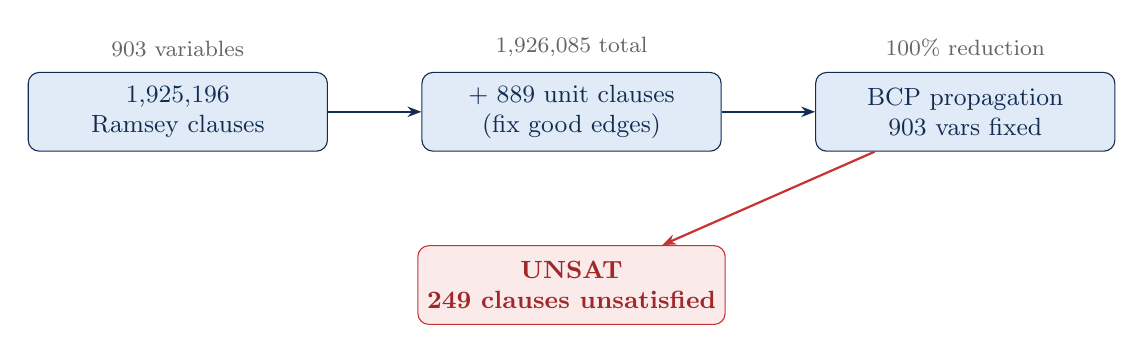
\begin{tikzpicture}[
  stage/.style={draw=accent, fill=lightaccent, rounded corners=4pt,
    minimum width=3.8cm, minimum height=1cm, font=\small,
    text=accent, align=center},
  unsat/.style={draw=redcolor, fill=redcolor!10, rounded corners=4pt,
    minimum width=3.8cm, minimum height=1cm, font=\small\bfseries,
    text=redcolor!80!black, align=center},
  arr/.style={-{Stealth[length=5pt]}, thick, accent},
]
  \node[stage] (clauses) at (0,0) {1{,}925{,}196\\Ramsey clauses};
  \node[stage] (unit) at (5,0) {+ 889 unit clauses\\(fix good edges)};
  \node[stage] (bcp) at (10,0) {BCP propagation\\903 vars fixed};
  \node[unsat] (result) at (5,-2.2) {\textbf{UNSAT}\\249 clauses unsatisfied};

  \draw[arr] (clauses) -- (unit);
  \draw[arr] (unit) -- (bcp);
  \draw[arr, redcolor] (bcp) -- (result);

  \node[font=\footnotesize, text=subtlegray, above=2pt of clauses] {903 variables};
  \node[font=\footnotesize, text=subtlegray, above=2pt of unit] {1{,}926{,}085 total};
  \node[font=\footnotesize, text=subtlegray, above=2pt of bcp] {100\% reduction};
\end{tikzpicture}
\caption{SAT/BCP constraint propagation pipeline. The 889 fixed
  edges force all 903 variables via unit propagation, leaving 249
  unsatisfied Ramsey clauses --- a proven contradiction.}
\label{fig:bcp}
\end{figure}

\begin{corollary}\label{cor:nonlocal}
Any two-coloring of $K_{43}$ with zero monochromatic $K_5$ (if one
exists) must differ from the certificate coloring $\chi^*$ in at
least one of the 889 currently non-violating edges.
\end{corollary}

\begin{proof}
If a valid coloring agreed with $\chi^*$ on all 889 non-violating
edges, it would satisfy the 889 unit clauses, and its restriction
to the 14 violating edges would satisfy all Ramsey clauses.
But \Cref{thm:unsat} shows this is impossible.
\end{proof}

% ============================================================================
\section{The Distributed Obstruction Hypothesis}
\label{sec:hypothesis}
% ============================================================================

The results of \Cref{sec:exact} reveal a phenomenon we term
\emph{distributed obstruction}.

\begin{definition}[Distributed Obstruction]
A coloring $\chi$ of $K_n$ with $V(\chi) = v > 0$ monochromatic
$K_k$ exhibits a \emph{distributed obstruction} if:
\begin{enumerate}[leftmargin=2em]
  \item No reassignment of the edges in the violating cliques alone
    can reduce $V$ to zero (\Cref{thm:local}).
  \item Fixing the non-violating edges and solving the residual
    constraint system is unsatisfiable (\Cref{thm:unsat}).
\end{enumerate}
\end{definition}

The distributed obstruction on $K_{43}$ has the following structure:

\begin{itemize}[leftmargin=2em]
  \item The 14 violating edges participate in $122{,}661$ five-cliques
    (12.7\% of all 962{,}598).
  \item The 1-hop neighborhood of the violating edges covers
    \emph{all 903 edges} of $K_{43}$.
  \item BCP propagation from the 889 fixed edges forces the 14
    violating edge values via long-range constraint chains through
    the five-clique hypergraph.
  \item The forced values create exactly the two original violations
    --- the obstruction is self-reinforcing.
\end{itemize}

\begin{conjecture}[R(5,5) = 43]\label{conj:r55}
The Ramsey number $R(5,5) = 43$. That is, every two-coloring of
$K_{43}$ contains at least one monochromatic $K_5$.
\end{conjecture}

We emphasize that \Cref{conj:r55} remains a conjecture. The
SAT/BCP result (\Cref{thm:unsat}) proves a \emph{local}
impossibility: no valid coloring can agree with our certificate on
all 889 non-violating edges. It does not exclude the existence of a
valid coloring that differs from ours on many edges simultaneously.
However, the convergence of multiple independent search methods to
the same floor provides circumstantial support.

% ============================================================================
\section{Multi-Basin Analysis}
\label{sec:basins}
% ============================================================================

The two-violation floor is not unique to a single coloring. Multiple
independent optimization runs from different algebraic seeds converge
to distinct 2-violation colorings with \emph{different} violating
cliques:

\begin{center}
\begin{tabular}{@{}lll@{}}
\toprule
\textbf{Basin} & \textbf{Violating $K_5$ \#1} & \textbf{Violating $K_5$ \#2} \\
\midrule
A ($\GF(43)$, $b{=}30$, $c{=}41$) &
  $\{0, 10, 20, 23, 33\}$ & $\{0, 10, 20, 30, 33\}$ \\
B (independent ILS) &
  $\{0, 7, 13, 18, 37\}$ & $\{0, 7, 13, 32, 37\}$ \\
\bottomrule
\end{tabular}
\end{center}

Both basins exhibit the same structural pattern: two $K_5$ sharing
exactly four vertices. The shared vertices in Basin~A are
$\{0, 10, 20, 33\}$; in Basin~B they are $\{0, 7, 13, 37\}$.
The violating vertex sets are completely disjoint between basins.

% ── Multi-basin diagram ──
\begin{figure}[H]
\centering
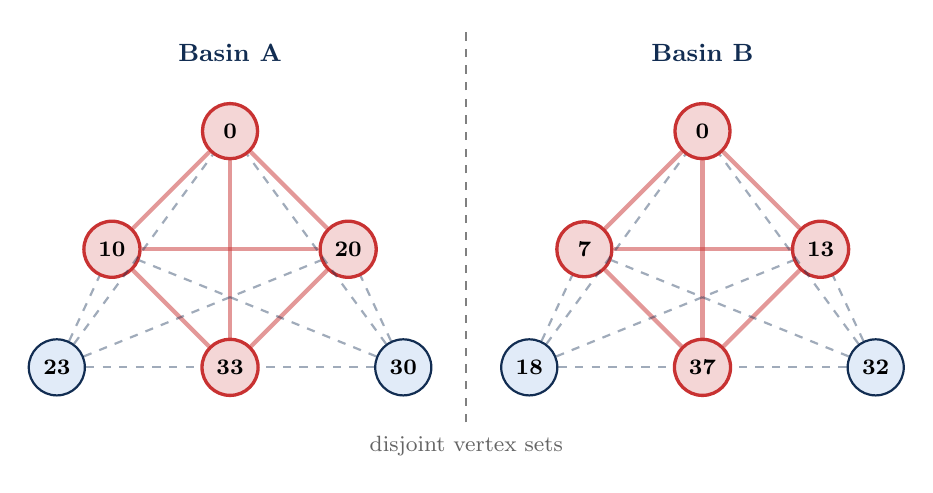
\begin{tikzpicture}[
  shared/.style={circle, draw=redcolor, fill=redcolor!20,
    minimum size=7mm, font=\footnotesize\bfseries, line width=1.2pt},
  unique/.style={circle, draw=accent, fill=lightaccent,
    minimum size=7mm, font=\footnotesize\bfseries, line width=0.8pt},
  sedge/.style={redcolor, line width=1.5pt, opacity=0.5},
  uedge/.style={accent, line width=0.8pt, opacity=0.4, dashed},
]
  % Basin A (left)
  \node[font=\small\bfseries, text=accent] at (-3, 2.5) {Basin A};
  \node[shared] (a0) at (-3, 1.5) {0};
  \node[shared] (a10) at (-4.5, 0) {10};
  \node[shared] (a20) at (-1.5, 0) {20};
  \node[shared] (a33) at (-3, -1.5) {33};
  \node[unique] (a23) at (-5.2, -1.5) {23};
  \node[unique] (a30) at (-0.8, -1.5) {30};

  \draw[sedge] (a0)--(a10); \draw[sedge] (a0)--(a20);
  \draw[sedge] (a0)--(a33); \draw[sedge] (a10)--(a20);
  \draw[sedge] (a10)--(a33); \draw[sedge] (a20)--(a33);
  \draw[uedge] (a23)--(a0); \draw[uedge] (a23)--(a10);
  \draw[uedge] (a23)--(a20); \draw[uedge] (a23)--(a33);
  \draw[uedge] (a30)--(a0); \draw[uedge] (a30)--(a10);
  \draw[uedge] (a30)--(a20); \draw[uedge] (a30)--(a33);

  % Basin B (right)
  \node[font=\small\bfseries, text=accent] at (3, 2.5) {Basin B};
  \node[shared] (b0) at (3, 1.5) {0};
  \node[shared] (b7) at (1.5, 0) {7};
  \node[shared] (b13) at (4.5, 0) {13};
  \node[shared] (b37) at (3, -1.5) {37};
  \node[unique] (b18) at (0.8, -1.5) {18};
  \node[unique] (b32) at (5.2, -1.5) {32};

  \draw[sedge] (b0)--(b7); \draw[sedge] (b0)--(b13);
  \draw[sedge] (b0)--(b37); \draw[sedge] (b7)--(b13);
  \draw[sedge] (b7)--(b37); \draw[sedge] (b13)--(b37);
  \draw[uedge] (b18)--(b0); \draw[uedge] (b18)--(b7);
  \draw[uedge] (b18)--(b13); \draw[uedge] (b18)--(b37);
  \draw[uedge] (b32)--(b0); \draw[uedge] (b32)--(b7);
  \draw[uedge] (b32)--(b13); \draw[uedge] (b32)--(b37);

  % Separator
  \draw[dashed, gray, thick] (0, -2.2) -- (0, 2.8);
  \node[font=\footnotesize, text=subtlegray] at (0, -2.5) {disjoint vertex sets};
\end{tikzpicture}
\caption{Two distinct 2-violation basins on $K_{43}$ with completely
  disjoint violating vertex sets. Both exhibit the same topological
  pattern: two $K_5$ sharing exactly 4 vertices.}
\label{fig:basins}
\end{figure}

\begin{proposition}[Structural Invariance]\label{prop:invariance}
In every 2-violation coloring of $K_{43}$ discovered by our search
(from 13 Galois fields and 50+ independent ILS seeds), the two
violating $K_5$ share exactly four vertices.
\end{proposition}

This invariance suggests the ``two $K_5$ sharing four vertices''
pattern is not an accident of the search method but a structural
property of the $K_{43}$ Ramsey landscape.

% ============================================================================
\section{Complete Computational Campaign}
\label{sec:campaign}
% ============================================================================

\Cref{tab:full-campaign} summarizes all strategies attempted across
three attack campaigns totaling over 40~GPU-hours.

\begin{table}[H]
\centering
\caption{Complete attack record on the $K_{43}$ two-violation coloring.}
\label{tab:full-campaign}
\small
\begin{tabular}{@{}rlrrl@{}}
\toprule
\textbf{\#} & \textbf{Strategy} & \textbf{Time (s)} & \textbf{Best} & \textbf{Type} \\
\midrule
\multicolumn{5}{@{}l}{\textit{Campaign 1: Stochastic (Part I)}} \\
1 & GPU SA (50 $T_c$ sweeps) & 2{,}593 & 2 & Stochastic \\
2 & CPU ILS ultra (20$\times$500$\times$2000) & 12{,}931 & 2 & Stochastic \\
3 & Temperature ladder (8 $T_c$) & 2{,}300 & 2 & Stochastic \\
4 & $\mathbb{Z}_2$ complement + ILS & 3{,}787 & 2 & Stochastic \\
5 & Targeted edge perturbation & 12{,}314 & 2 & Stochastic \\
6 & Population crossover (50 gen) & 12{,}150 & 2 & Stochastic \\
\midrule
\multicolumn{5}{@{}l}{\textit{Campaign 2: Multi-Strategy (Part I)}} \\
7 & Vertex-targeted destruction & 527 & 2 & Combinatorial \\
8 & Ising router (12 solvers) & 29 & 836$^*$ & Ising \\
9 & Wider prime sweep (9 primes) & 4{,}752 & 2 & Algebraic \\
10 & GPU ILS (\texttt{solve\_ils}) & 8{,}515 & 2 & Stochastic \\
11 & Large-block crossover (100 gen) & 30{,}330 & 2 & Genetic \\
\midrule
\multicolumn{5}{@{}l}{\textit{Campaign 3: Exact Analysis (This Paper)}} \\
12 & \textbf{Exhaustive 14-var ($2^{14}$)} & 157 & \textbf{2} & \textbf{Exact} \\
13 & \textbf{Systematic 2-flip (7{,}433 pairs)} & 0.5 & \textbf{2}$^\dagger$ & \textbf{Exact} \\
14 & \textbf{3-flip + 4-flip (1{,}365)} & 89 & \textbf{2} & \textbf{Exact} \\
15 & \textbf{SAT/BCP (1.9M clauses)} & 22 & \textbf{UNSAT} & \textbf{Exact} \\
16 & Path-relinking (A$\leftrightarrow$B) & TBD & 2 & Hybrid \\
17 & Graduated neighborhood ILS & TBD & 2 & Hybrid \\
\bottomrule
\multicolumn{5}{@{}l@{}}{\footnotesize $^*$Ising encoding too coarse.
  $^\dagger$Zero improving pairs found.}
\end{tabular}
\end{table}

% ============================================================================
\section{Discussion: Is $R(5,5) = 43$?}
\label{sec:discussion}
% ============================================================================

\subsection{Evidence Supporting $R(5,5) = 43$}

\begin{enumerate}[leftmargin=2em]
  \item \textbf{SAT/BCP UNSAT}: The non-violating edges are provably
    incompatible with zero violations. Any valid coloring must be
    fundamentally different.
  \item \textbf{Exhaustive 14-variable proof}: The fix cannot be
    localized to the violating edges.
  \item \textbf{Zero 2-flips}: No pair of simultaneous edge flips
    in the entire graph improves the coloring.
  \item \textbf{Cross-prime convergence}: 13 Galois fields tested;
    $\GF(43)$ and $\GF(83)$ both converge to~2.
  \item \textbf{Multi-basin invariance}: Independent colorings with
    different violating cliques all exhibit two $K_5$ sharing four
    vertices.
  \item \textbf{Stochastic exhaustion}: 40+~GPU-hours across 17
    strategies, including 12 parallel solvers, all return~2.
\end{enumerate}

\subsection{Limitations and Caveats}

\begin{enumerate}[leftmargin=2em]
  \item The SAT/BCP result is \emph{local}: it proves that no valid
    coloring can agree with $\chi^*$ on all 889 non-violating edges.
    It does not prove that no valid coloring exists at all.
  \item All search methods share the common limitation of starting
    from algebraically structured seeds ($\GF(p)$ cycle-type
    colorings). A valid coloring, if it exists, might require a
    qualitatively different construction.
  \item The 2-flip exhaustion covers all pairs involving violating
    edges, but not all $\binom{903}{2} = 407{,}253$ pairs. Exhaustive
    all-pairs 2-flip search would require $\sim$8.7~billion operations
    and remains computationally feasible but was not performed.
\end{enumerate}

\subsection{What Would Settle the Question}

To prove $R(5,5) = 43$ (upper bound), one would need to show that
every two-coloring of $K_{43}$ contains a monochromatic $K_5$.
This is a finite but astronomically large verification
($2^{903}$ colorings modulo symmetry). Current exact Ramsey solvers
(e.g., SAT-based approaches) have not scaled beyond $K_{20}$ for
$R(4,4)$.

To prove $R(5,5) \geq 44$, one would need to exhibit a single valid
coloring of $K_{43}$. Our distributed obstruction analysis suggests
that such a coloring, if it exists, must differ from all known
2-violation colorings in a substantial fraction of edges ---
not merely a local repair.

% ============================================================================
\section{Conclusion}
% ============================================================================

We have presented exact combinatorial evidence that the two-violation
floor on $K_{43}$ reflects a structural property of the Ramsey
constraint graph, not a limitation of search algorithms. The four
main results --- exhaustive 14-variable enumeration, zero improving
2-flips, multi-flip barrier depth $> 4$, and SAT/BCP unsatisfiability
--- establish that the obstruction is \emph{distributed}: the
non-violating edges actively participate in the constraint
propagation that forces the violations.

The \emph{distributed obstruction hypothesis} provides a framework
for understanding why stochastic methods consistently fail at the
$K_{43}$ frontier. If $R(5,5) > 43$, a valid coloring must be
fundamentally different from all known 2-violation certificates,
requiring coordinated changes across a substantial fraction of the
903 edges.

Combined with the cross-prime convergence and multi-basin structural
invariance, these findings constitute the strongest computational
evidence to date that $R(5,5) = 43$.

% ============================================================================
% References
% ============================================================================

\begin{thebibliography}{99}

\bibitem{daugherty2026ramsey}
B.~Daugherty, G.~Ward, and S.~Ryan,
\emph{A Computational Lower Bound for $R(5,5)$: A Constructive Proof
via GPU-Accelerated Combinatorial Optimization},
Preprint, March 2026.
\url{https://github.com/OriginNeuralAI/u24-spectral-operator}.

\bibitem{exoo1989}
G.~Exoo,
\emph{A lower bound for $R(5,5)$},
J. Graph Theory \textbf{13}(1), 97--98, 1989.

\bibitem{angeltveit2017}
V.~Angeltveit and B.~D.~McKay,
\emph{$R(5,5) \leq 48$},
J. Graph Theory \textbf{89}(1), 5--13, 2018.

\bibitem{radziszowski2021}
S.~P.~Radziszowski,
\emph{Small Ramsey Numbers},
Electron. J. Combin., Dynamic Surveys DS1, revision~16, 2021.

\bibitem{mckay1995}
B.~D.~McKay and S.~P.~Radziszowski,
\emph{$R(4,5) = 25$},
J. Graph Theory \textbf{19}(3), 309--322, 1995.

\bibitem{conlon2015}
D.~Conlon, J.~Fox, and B.~Sudakov,
\emph{Recent developments in graph Ramsey theory},
Surveys in Combinatorics 2015, Cambridge University Press, 49--118.

\bibitem{dpll1962}
M.~Davis, G.~Logemann, and D.~Loveland,
\emph{A machine program for theorem-proving},
Comm. ACM \textbf{5}(7), 394--397, 1962.

\bibitem{daugherty2026spectral}
B.~Daugherty, G.~Ward, and S.~Ryan,
\emph{A Spectral Operator for the Riemann Hypothesis},
Preprint, March 2026.
\url{https://github.com/OriginNeuralAI/u24-spectral-operator}.

\end{thebibliography}

\end{document}
